%! TEX root=./main.tex
\section{Methods}

\subsection{Laboratory experimental design}

\subsubsection{BUILD: Construction of genetic devices}

\textbf{Plasmid Design.}
The pBbB6c-GFP plasmid has been used for all our designs.
This plasmid comes with GFP mut3b CDS inducible with addition of isopropyl $\beta$-D-1-thiogalactopyranoside (IPTG).
The original RBS for the GFP CDS was replaced with combination of PCR and isothermal assembly.
Primers and the assembly strategy have been generated using the Teselagen DESIGN software (Teselagen Biotechnology).

\textbf{PCR.}
PCR amplification of the cloning inserts was done using Q5 High-Fidelity 2X Master Mix (NEB, catalogue no. M0492L).
20 $\mu$L reactions were prepared by dispensing \hl{1 $\mu$L of each 10 $\mu$M reverse primer into the wells} of a 96-well PCR plate using the Labcyte Echo Liquid Handler.
A mastermix consisting of polymerase premix, plasmid DNA template \hl{(pBbB6C, 5-10 ng per reaction)}, and the single 10 $\mu$M forward primer was prepared by and dispensed \hl{using the FeliX liquid handler or electronic multi-channel pipette}. Reactions were run using Touchdown PCR or standard PCR cycling methods in BioRad C1000 thermal cyclers.
Capillary electrophoresis of PCR products was performed using the Agilent Technologies ZAG DNA Analyzer system.
2 $\mu$L of each PCR reaction was electrophoresed using the ZAG 130 dsDNA Kit (75-20000bp) or ZAG 110 dsDNA Kit (35-5000bp) (Agilent Technologies, catalogue no. ZAG-110-5000; ZAG-130-5000). \hl{ZAG sample plates were prepared using the Perkin Elmer Sciclone G3 liquid handler.}
ProSize Data Analysis Software (Agilent Technologies) was used to generated gel images from the sample chromatograms and sizes were estimated by reference to the upper and lower DNA markers spiked into each sample and a DNA ladder run in well H12 of each sample plate. 

\textbf{Isothermal DNA Assembly.}
Constructs were assembled using NEBuilder HiFi DNA Assembly Master Mix (NEB, catalogue no. E2621L).
Reactions consisting of \hl{approximately equal amounts} of the common fragment and the variable fragment were prepared \hl{using the FeliX liquid handler or electronic multi-channel pipette}, to a final volume of 5 or 10 $\mu$L.
Assemblies were run in the thermal cycler for 1 hour at 50$^{\circ}$C, followed by an infinite hold step at 4$^{\circ}$C.
Finally, samples were \hl{incubated with of 50 nL of DpnI (NEB, catalogue no. R0176S) at 37$^{\circ}$C for 90 minutes to remove any residual template DNA.}

\textbf{\textit{E. coli} transformation.}
The DH5$\alpha$ cell line (Thermo Fisher Scientific, catalogue no. 18265017) was made chemically competent using the Mix $\&$ Go \textit{E. coli} Transformation Kit $\&$ Buffer Set (Zymo Research, catalogue no. T3001).
20 $\mu$L of cells was aliquoted into each well of a cold 96-well PCR plate and stored at -80$^{\circ}$C for later use.
Plates of cells were thawed on a -20$^{\circ}$C cold block before 3 $\mu$L of the assembly product was added and mixed using the CyBio FeliX liquid handler.
Cells were incubated on a cold block for 2-5 minutes before being plated in a 96 \hl{(12 x 8)} grid on Omnitrays containing LB (BD, catalogue no. 244610) and 15 g/L agar (Sigma-Aldrich, catalogue no. A1296) with 34 $\mu$g/mL chloramphenicol (Sigma-Aldrich, catalogue no. C1919).
Plates were incubated overnight at 37$^{\circ}$C. \hl{Cells were plated using the CyBio FeliX liquid handler.}

\textbf{Automated colony picking and culturing.}
A Singer Instruments PIXL colony picker was used to select individual colonies from the transformation plates using the 490-510 nm (cyan) light filter.
Each selected colony was used to inoculate 1 mL of selective medium in a 2 mL square well 96 plate.
They were then cultured overnight in 37$^{\circ}$C with shaking (~300 rpm).

\textbf{Glycerol stock preparation.}
100 $\mu$L of sterile 80\% (v/v) glycerol (Chem-Supply, catalogue no. GA010) and 100 $\mu$L of overnight culture were combined in the wells of a 96 deep (2 mL) round well plate \hl{using the CyBio FeliX liquid handler or electronic multichannel pipette}
They were then sealed with a 96-well silicone sealing mat and transferred to a -80$^{\circ}$C freezer. 

\textbf{Sequencing}
Strains that gave GFP fluorescence intensity readings similar to that of the original RBS were selected for sequence confirmation by capillary electrophoresis sequencing (CES) by Macrogen, Inc. (Seoul, South Korea).
The strains transformed with each of the selected constructs were grown to saturation in 5 mL LB medium with chloramphenicol selection (34 $\mu$g/mL).
Plasmids were extracted from the cultures using the QIAprep Spin Miniprep Kit (QIAGEN, catalogue no. 27106) according to the manufacturer's instructions.
Plasmid concentrations were quantified using the Cytation 5 plate reader with the Take3 Micro-Volume Plate (BioTek) and all fell in the range of 100-200 ng/$\mu$L.
Samples of 20 $\mu$L of undiluted plasmid DNA were sequenced using a single primer (5'-CGATATAGGCGCCAGCAA-3') that binds approximately 150 bp upstream of the RBS.
Reads were aligned with the template sequence in the Teselagen software (TeselaGen Biotechnology, Inc.).

\subsubsection{TEST: Culture analysis}

\textbf{Test strain culture.}
Overnight cultures were started by inoculating 1 mL of LB medium supplemented with 34 $\mu$g/mL chloramphenicol with ~2 $\mu$L of the glycerol stock in a 96 deep (2 mL) round well plate, \hl{using the CyBio FeliX liquid handler or electronic multichannel pipette}
Cultures were incubated at 37$^{\circ}$C with shaking (~300 rpm) for ~17 hours. 
The following morning, 20 $\mu$L of overnight cultures were added to 980 $\mu$L of fresh selection medium and these cultures were grown at 37$^{\circ}$C with shaking in 2 mL round well 96 plate. 
\hl{After 90 minutes, cultures were induced with IPTG (Sigma-Aldrich, catalogue no. I5502) to a final concentration of 0.5 mM. This was done by transferring 1.0 $\mu$L of 0.1M IPTG to each well of a flat-bottom clear polystyrene 96-well plate using the Echo acoustic liquid handler, then adding 300 $\mu$L of culture to each well using an electronic multichannel pipette}

\textbf{Microplate spectrophotometry.}
The plates were monitored in the Cytation 5 microplate reader immediately after the addition of IPTG.
Cytation 5 acquisition and incubation/shaking settings were as follows: length of run: \hl{8 hours}; interval: 10 min; continuous orbital shake at 237 rpm and slow orbital speed; excitation wavelength: 490/10 nm; emission wavelength: 515/10 nm; bottom read; gain: 60; read height: 7 mm; read speed: Sweep.

\subsection{Machine learning experimental design}

Two types of machine learning algorithms can be applied to drive the experimental design workflow shown in Figure \ref{fig: Flowchart}.
% To automatically design the RBS sequences in batch using machine learning, we can logically divided the workflow into two parts: 
One type of machine learning algorithms is a prediction algorithm (\textbf{LEARN}), which helps us learn the function of TIR with respect to RBS sequences. The other type of machine learning algorithm is a recommendation algorithm (\textbf{DESIGN}), which recommends RBS sequences to query (test) in each round (in the sense of a single pass through the DBTL cycle) based on the predictions from LEARN. \\

% 1) \textbf{LEARN}: A regression algorithm which takes the RBS sequences as input features and TIR scores as labels, trains on sequences with known labels and returns the predicted TIR scores and the respective confidence intervals.
% 2) \textbf{DESIGN}: An online learning approach which recommends the RBS sequences based on the predicted TIR scores and confidence intervals.
In round $t$, the prediction and design is based on the results obtained in all previous rounds. 
Our implementation of the machine learning algorithms was tested in Python 3.6 and used the scikit-learn library \cite{scikit-learn}. 
In the following paragraphs, we describe our machine learning pipeline \hl{(which is applicable to design rounds 1-3, denoted as Bandit 1-3)} in the following order: data pre-processing, prediction and kernels and finally recommendation. 
\hl{The pipeline for our 0th round of designs, denoted as Bandit-0, is reported in Supplementary} \ref{sec: ML design pipeline}.

\subsubsection{Data pre-processing}
\label{sec: method data pre-procesing}

\hl{For each RBS sequence, we measured the TIR of 6 biological replicates, where TIR is calculated as a derivative of GFP fluorescence divided by OD600 of culture over time, following the formula:}

$$\mathnormal{TIR=\int_{t_{min}}^{t_{max}}\frac{GFP}{OD_{600}}dt}$$

\hl{where ${t_{min}}$ is time at which $\frac{GFP}{OD_{600}}$ value is minimum denoting start of the log growth phase and ${t_{max}}$ is time at which the logarithmic phase ends (on average, for our samples that was at 4h from ${t_{min}}$ and so that was the time point used for TIR calculations for all samples).}\\

% REVIEW:
% \mengyan{Table XXX shows an example of our raw data. }
% We consider both the label (TIR) pre-processing and kernel pre-processing.
For label pre-processing, we first adjust the TIR values in each round using the round-wise reference values.
This reference values are the TIR of the benchmark sequence that is run in triplicate in each round.
Specifically, in round $t$, we subtract the TIR mean of the benchmark RBS measured in round $t$ from all TIR values measured in the same round, for each replicate separately. 
We then normalised the data by performing a logarithm transformation and standardisation on the adjusted TIR label for each replicate separately.
After normalisation, each replicate has zero mean and unit variance. 
Furthermore, we also normalised the kernel matrix used for prediction by centring and unit-norm normalisation, which is reviewed in details in Supplementary \ref{supp: Normalisation of Kernel}.
% Since the design space is known, we consider the transductive approach \cite{} for the kernel pre-processing with centering and unit-norm normalisation. 


\subsubsection{Prediction: Gaussian Process Regression with String Kernel}
\label{sec: method prediction with kernel}

To find RBS sequences with the highest possible TIR score after a total number of rounds $N$,  we consider our experimental design problem as a sequential optimisation of an unknown reward function $f: \mathcal{D} \rightarrow \mathbb{R}$, where $\mathcal{D}$ is the set containing all RBS sequence points in the design space, and $f(\mathbf{x})$ \hl{is the TIR score of the 6-base core sequence considered in its wider 20-base full RBS sequence $\mathbf{x} \in \{A,C,G,T\}^{20}$}.
In each round $t$, we choose a set of $m$ points $\mathcal{S}_t \subset \mathcal{D}$ and observe the function value at each point in the selected set $\mathcal{S}_t$, i.e. $y_i = f(\mathbf{x}_i) + \epsilon$, for all $i \in \mathcal{S}_t$, where $\epsilon$ is the Gaussian random noise with unknown mean and variance. \\
% This noise is influenced by the accuracy of the RBS predictor and other experimental sources of interference (e.g. time, temperature, operator, etc.). 
% REVIEW:
% \mengyan{we should discuss measurement noise somewhere, maybe with a sample example for the dataset we used.}

For regression model, we have used a Bayesian non-parametric approach called \textit{Gaussian Process Regression (GPR)} \cite{Rasmussen2004,srinivas2012information, romero_navigating_2013}.
We model $f$ as a sample from a \textit{Gaussian Process} $\mathcal{G} \mathcal{P}(\mu(\mathbf{x}), k(\mathbf{x}, \mathbf{x'}))$, which is specified by the mean function $\mu(\mathbf{x})=\mathbb{E}[f(\mathbf{x})]$ and the kernel function (also called \textit{covariance function}) $k\left(\mathbf{x}, \mathbf{x}^{\prime}\right)=\mathbb{E}[(f(\mathbf{x})-\left.\mu(\mathbf{x}))\left(f\left(\mathbf{x}^{\prime}\right)-\mu\left(\mathbf{x}^{\prime}\right)\right)\right]$.
%As illustrated in Figure \ref{fig: Gaussian Process Regression Example.}, 
GPR can predict both the posterior mean and standard deviation \hl{of the RBS sequences in the design space}. The posterior standard deviation represents the level of uncertainty for the prediction. 
We review the predictions of GPR in Supplementary \ref{supp: GPR}.\\
% We assume the observations are noisy, so even when a data point in observed then confidence interval is still bigger than 0. 
% As we can see, the true function is in the confidence interval when there are data points are observed. 

% \begin{figure}[t]
%     \centering
%     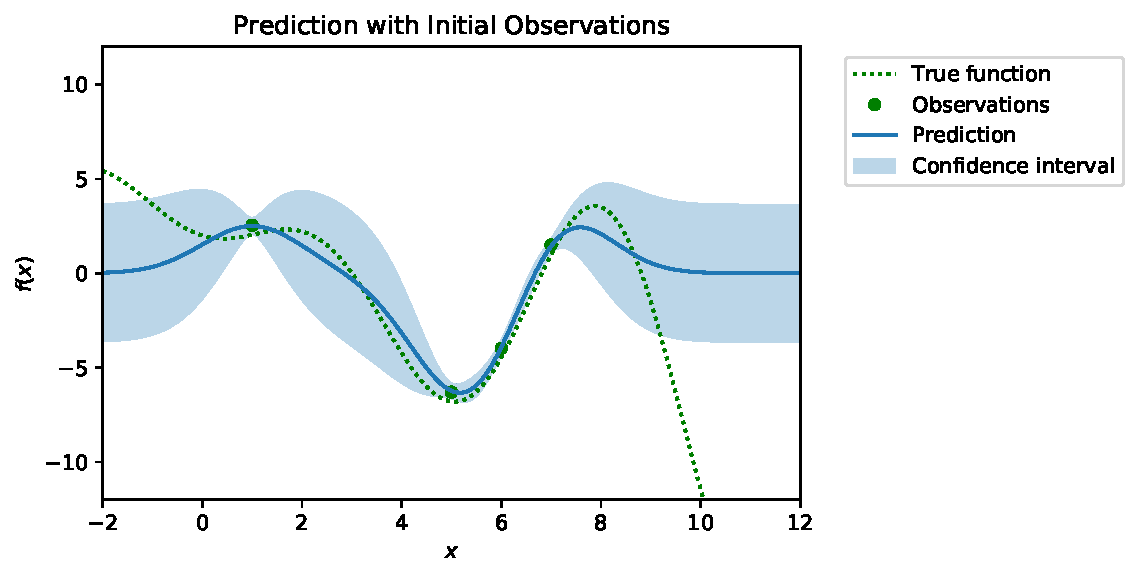
\includegraphics[scale=0.7]{plots/Prediction with Initial Observations.pdf}
%     \caption{Gaussian Process Regression Example. This plot shows the GPR prediction with confidence interval based on 4 initial observations. The confidence interval are shown in predicted mean $\pm$ 1.96 standard deviation.}
%     \label{fig: Gaussian Process Regression Example.}
% \end{figure}

The choice of kernel function is critical for accurate predictions, since it controls smoothness and amplitude of the function to be modelled.
For Bandit designs in Round 0, since we only had access to limited number of data points from literature, we chose to use one of the basic string kernels, the \textit{spectrum kernel} \cite{leslie2001spectrum} to process the core 6bp and dot product kernel \cite{Rasmussen2004} (with one-hot embedding) to process the 7bp flanking sequences both upstream and downstream of the core sequence.
To represent the RBS sequences in subsequent rounds, we use the \textit{weighted degree kernel with shift} (WDS) \cite{ratsch_rase_2005_wds,Ben-Hur2008} to specify the kernel function of $GP$.  
WDS is a type of a string kernel, which takes two sequences as inputs and outputs a scalar value which represents the similarities between the two sequences.  
WDS kernel does this by counting the matches of substrings of a certain length (i.e. kmers) that constitute the sequence.
The maximum substring length is specified by $\ell$. 
The WDS takes into account the positional information by counting substrings starting from different positions, where the start position is specified by $l$.
Additionally, the WDS kernel considers the shifting of substrings, with the maximum shift specified by $s$.
This could be useful when there is a shift between two sequences.
For example, two sequences A\textbf{CCTGA} and \textbf{CCTGA}A are in 1-shift. \\
% there is a common part \textbf{CCTGA} which is begins at the 2nd nucleotide in sequence 1 and at the 1st nucleotide in sequence 2, hence the calculated shift would be 1.

We now define WDS kernel. 
Let $\mathbb{I}$(A) be the indicator function, which equals 1 if $A$ is true and 0 otherwise. 
Then $\mathbb{I}(\mathbf{x}_{[l+s:l+s+d]} = \mathbf{x}_{[l:l+d]}^\prime)$ indicates whether two substrings of length $d$ match, between $\mathbf{x}$ starting from position $l+s$ and $\mathbf{x}^\prime$ starting from position $l$.
This is similarly done for $\mathbb{I}(\mathbf{x}_{[l:l+d]}= \mathbf{x}_{[l+s:l+s+d]}^\prime)$.
By having these two terms considering substrings of two sequences with starting positions differing by $s$ characters, the WDS can measure shifted positional information. 
When $s = 0$, the kernel function counts the matches with no shift between sequences. 
Let $\mathbf{x}, \mathbf{x}^\prime$ be two RBS sequences with length $L$, the WDS kernel is defined as
\begin{align}
        k_\ell^{WDS}(\mathbf{x}, \mathbf{x}^\prime) 
        %&= \sum_{d=1}^{\ell} \beta_d \sum_{l=1}^{L-d+1} \gamma_l \sum_{s = 0, s + l \leq L}^{S(l)} \delta_s
        %\left(k_d^{Spec}(\mathbf{x}_{[l+s:l+s+d]}, \mathbf{x}_{[l:l+d]}^\prime) + (k_d^{Spec}(\mathbf{x}_{[l:l+d]}, \mathbf{x}_{[l+s:l+s+d]}^\prime)\right)\\
        = \sum_{d=1}^{\ell} \beta_d \sum_{l=1}^{L-d+1} \gamma_l \sum_{s = 0, s + l \leq L}^{S(l)} \delta_s
        \left(\mathbb{I}(\mathbf{x}_{[l+s:l+s+d]} = \mathbf{x}_{[l:l+d]}^\prime) + \mathbb{I}(\mathbf{x}_{[l:l+d]}= \mathbf{x}_{[l+s:l+s+d]}^\prime)\right),
\end{align}
where 
$\beta_d = \frac{2(\ell - d + 1)}{\ell(\ell+1)}, \delta_s = \frac{1}{2(s+1)}$, $\gamma_l$ is a weighting parameter over the position in the
sequence, where we chose to use a uniform weighting over the sequences, i.e. $\gamma_l = 1/L$ ($L = 20$ in our design).
$S(l)$ determines the maximum shift at position $l$. 
Furthermore, we normalise the kernel with centring and unit norm in terms of all sequences in the design space. 
% In our design, the length of RBS sequence $L = 20$.
The hyperparameters for kernel, including maximum substring length $\ell$, maximum shift length $S(l)$, and the standard deviation of GP noise $\alpha$ were chosen based on 10-repeat 5-fold cross validation.
% ($\ell=6$, and $S(l)= 1$, $\alpha = 2$). 


    
    
%  For recommendations, we consider the \textit{Upper Confidence Bound (UCB)} type algorithms. 
%  As one popular type of the bandit algorithms \cite{lattimore2020bandit}, the UCB type of algorithms are based on the \textit{optimism in the face of uncertainty},
 %provide various approaches to sequential design where an agent adaptively chooses one or more options among several actions based on certain policies. In our work we used the Upper Confidence Bound version of that algorithm, which is based on the \textit{optimism in the face of uncertainty}. The UCB algorithm, as the name suggests,
%  which basically select RBS sequences with the maximum upper confidence bound constructed by the sum of the predicted mean and $n$ standard deviation ($n > 0$), i.e. $\operatorname{argmax}_{\mathbf{x}_i \in \mathcal{D}} \left( \mu_t(\mathbf{x}_i) + \beta_t \sigma_t(\mathbf{x}_i)\right)$,
%     where $\beta_t$ is a hyperparameter balancing the exploitation and exploration, 
%     $\mu_t(\mathbf{x}_i), \sigma_t(\mathbf{x}_i)$ are the predicted mean and standard deviation at round $t$ for the sequence $\mathbf{x}_i$. 

\subsubsection{Recommendation: Batch Upper Confidence Bound Bandit}

To recommend the RBS sequences to query in next round, we have used the \textit{Upper Confidence Bound (UCB)} batch algorithm \cite{srinivas2012information}, which provides  $\textit{exploitation-exploration balance}$.
On one hand, UCB exploits the function in terms of the design space, that is to pinpoint sequences that are believed to have high labels (i.e. high predicted mean); 
on the other hand, UCB explores the design space where we have little information and sequences have a chance to have high labels (i.e. high predicted standard deviation).
More precisely, UCB algorithm selects RBS sequence $\mathbf{x}_i \in \mathcal{D}$ with the maximum upper confidence bound at round $t$, i.e.
\begin{align}
\label{Eq: GPUCB}
    \operatorname{argmax}_{\mathbf{x}_i \in \mathcal{D}} \left( \mu_{t-1}(\mathbf{x}_i) + \beta_t \sigma_{t-1}(\mathbf{x}_i)\right),
\end{align}
where $\beta_t$ is a hyperparmeter balancing the exploitation and exploration, 
$\mu_t(\mathbf{x}_i), \sigma_t(\mathbf{x}_i)$ are the predicted mean and standard deviation at round $t$ for the sequence $\mathbf{x}_i$.
We call $\mu_{t-1}(\mathbf{x}_i) + \beta_t \sigma_{t-1}(\mathbf{x}_i)$ the \textit{UCB score} of sequence $\mathbf{x}_i$ at round $t-1$.\\

Since experimentally labelling sequences is time-consuming, it is unrealistic to recommend sequences sequentially (i.e. one-by-one) and then wait for the label to be tested and used to improve the model.
Instead, we can recommend RBS sequences in a batch of size $m$. 
One naive approach is to 
%train GP on sequences with known TIR labels and
recommend sequences in design space with top $m$ UCB scores, as shown in Figure \ref{fig:batch rec}A ($m = 2$).
However, this approach may end up recommending similar sequences in the same local maximum (e.g. $x = 2, x =2.5$ in this example). 
Since GPR assumes similar sequences would have similar labels (e.g. by knowing $x=2$ we can gain information about $x=2.5$ as well), we prefer to not to waste time and money on labelling sequences with high similarities in the same batch.
To counter this, we use a batch recommendation strategy that is designed to avoid recommending such highly similar sequences in the same batch, described below. \\

% \begin{figure}[t]
% \centering
% \subfloat{\label{main:c}\includegraphics[scale=.4]{plots/Recommend_2_Data_Point_Top_2_UCB.pdf}}\par\medskip
% \begin{minipage}{.5\linewidth}
% \centering
% \subfloat{\label{main:a}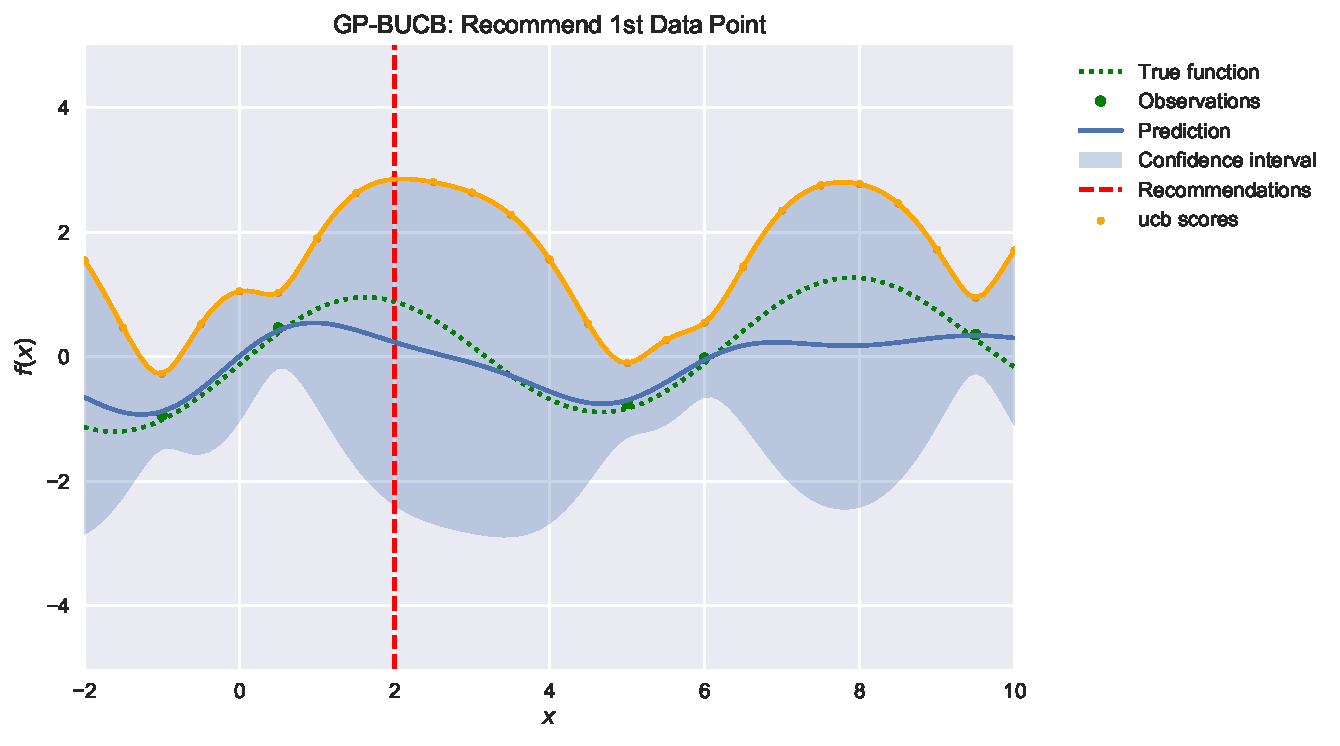
\includegraphics[scale=.4]{plots/GP-BUCB_Recommend_1st_Data_Point.pdf}}
% \end{minipage}%
% \begin{minipage}{.5\linewidth}
% \centering
% \subfloat{\label{main:b}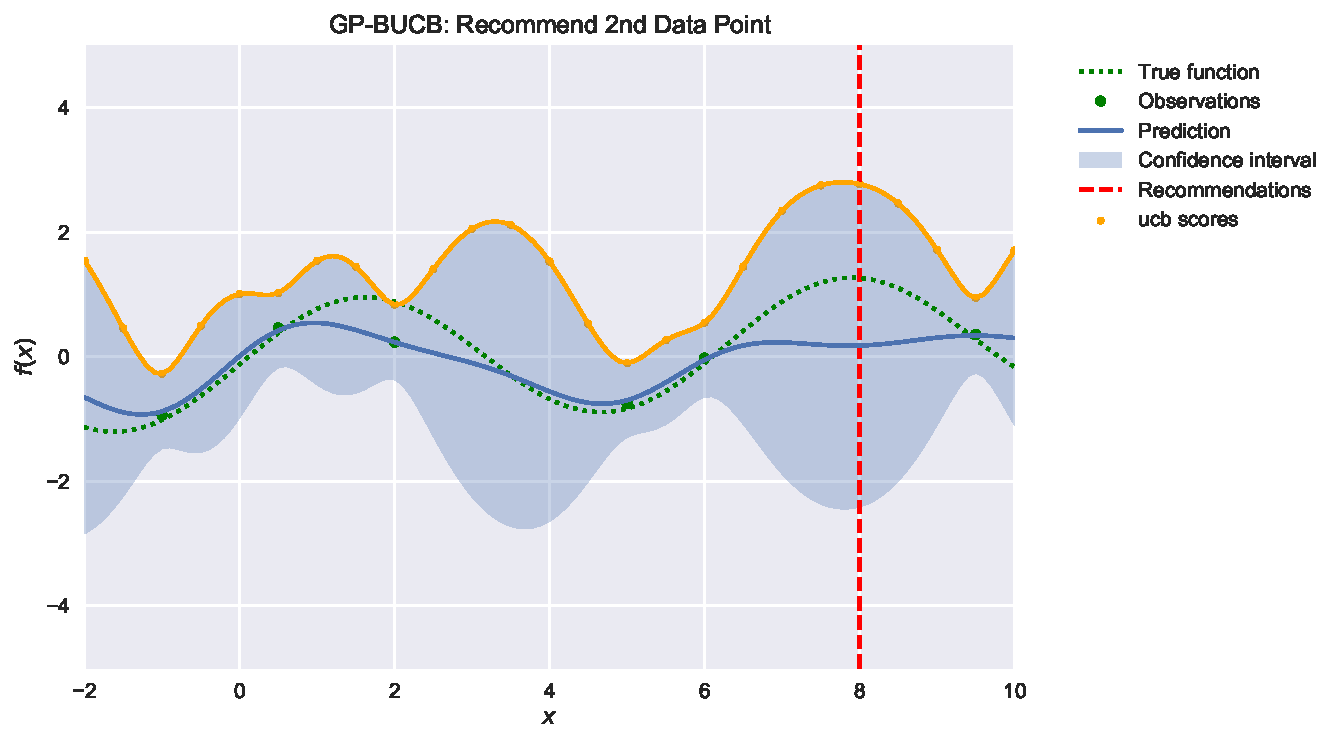
\includegraphics[scale=.4]{plots/GP-BUCB_Recommend_2nd_Data_Point.pdf}}
% \end{minipage}
% \caption{Batch Recommendation. We use the batch size of 2, with 5 initial observations. The design (recommendation) space is 24 uniformly distributed points in the range [-2,10], i.e. {-2, -1.5, -1, ..., 9.5, 10}.
% The confidence interval are shown with predicted mean of $\pm$ 1.96 standard deviation.
% (a) Top UCB recommendations. The recommendations are 2 data points with top UCB scores, constructed with GP predictions. 
% (b)(c) GP-BUCB recommendations. (b) shows the first recommended sequence, (c) shows the new predicted confidence interval and the second recommendation based on that.}
% \label{fig:batch rec}
% \end{figure}

\begin{figure}
    \centering
    \begin{subfigure}[b]{0.49\textwidth}
        \centering
        \caption{}
        \includegraphics[scale=.4]{plots/Main_Paper/Recommend_2_Data_Point_Top_2_UCB.pdf}
    \end{subfigure}
    \vskip\baselineskip
    \begin{subfigure}[b]{0.49\textwidth}
        \centering
        \caption{}
        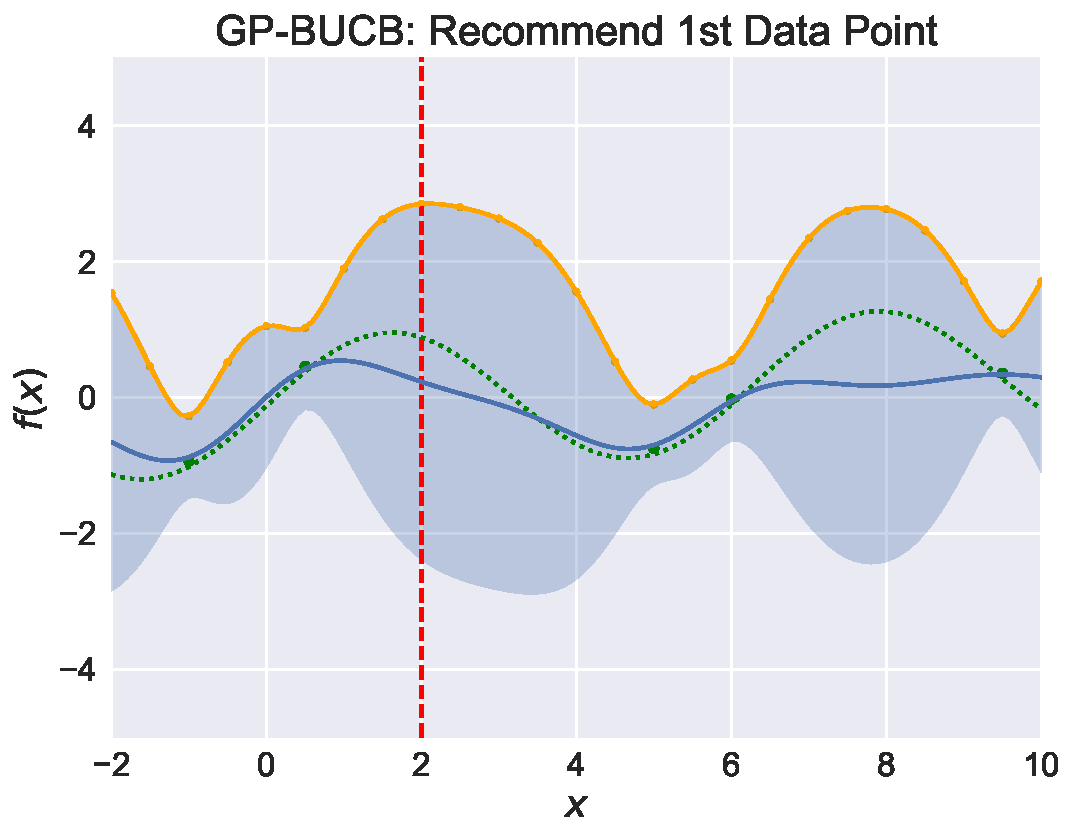
\includegraphics[scale=0.4]{plots/Main_Paper/GP-BUCB_Recommend_1st_Data_Point.pdf}
    \end{subfigure}
    \hfill
    \begin{subfigure}[b]{0.49\textwidth}
        \centering
        \caption{}
        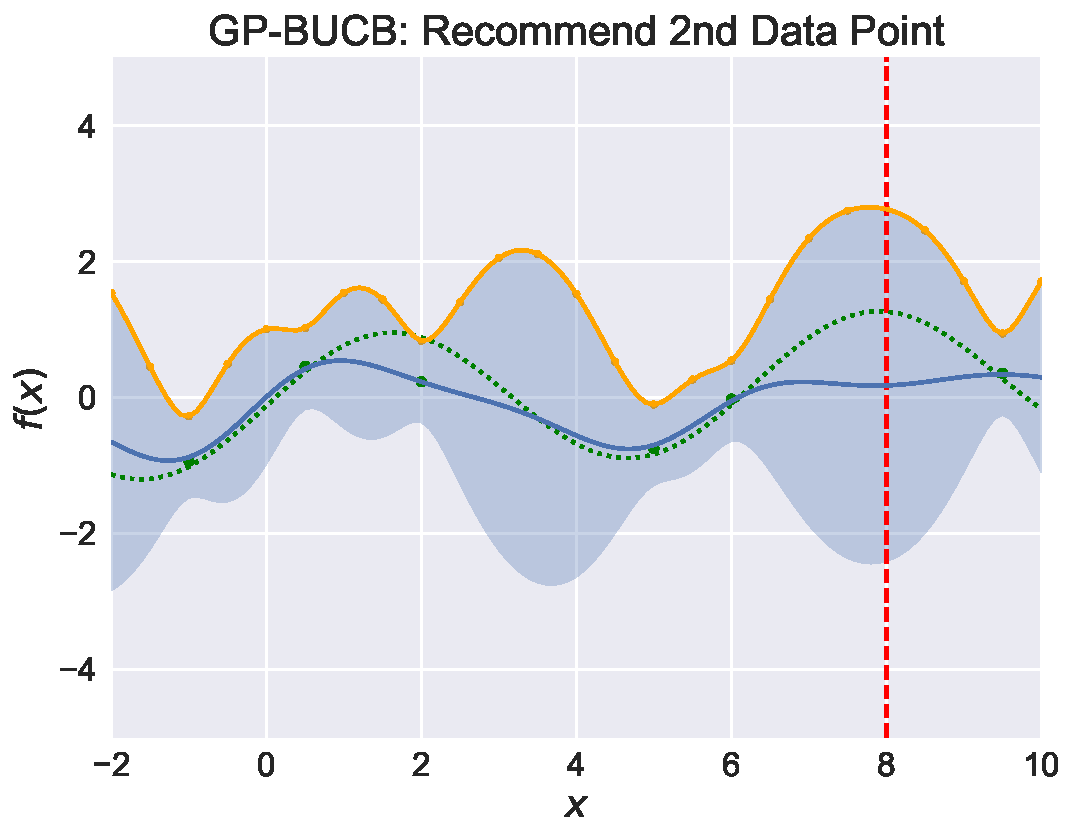
\includegraphics[scale=0.4]{plots/Main_Paper/GP-BUCB_Recommend_2nd_Data_Point.pdf}
    \end{subfigure}
    \caption{\emph{Batch Recommendation Illustration.} We use the batch size of 2, with 5 initial observations. The design space is 24 uniformly distributed points in the range [-2,10], i.e. {-2, -1.5, -1, ..., 9.5, 10}.
    The confidence intervals are shown with predicted mean $\pm$ 1.96 standard deviation.
    (A) Top UCB recommendations. The recommendations are 2 data points with top UCB scores, chosen with GP predictions. 
    (B)(C) Batch UCB recommendations. (B) shows the first recommended sequence, (C) shows the new predicted confidence interval and the second recommendation based on that updated interval.}
    \label{fig:batch rec}
\end{figure}


A key property of Gaussian Process regression is that the predicted standard deviation depends only on \hl{features}, not on the \hl{labels}. 
% We illustrate this fact by comparing the prediction with the true function value of the new recommended point (Figure \ref{fig: Recommend 1 Data Point (New Observation)}) and the prediction with the predicted value of the new recommended point (Figure \ref{fig: Recommend 1 Data Point (Predicted Mean)}).
% As we can see, the predicted confidence interval is the same for the two plots. 
One can make use of this property to design a batch upper confidence bound (BUCB) algorithm \cite{desautels2014parallelizing}.
The strategy here is to recommend \hl{RBS sequences one-by-one by sequentially adding the newly recommended RBS sequences into the training data and updating UCB scores.}\\
% Figure \ref{fig: Recommend 2 Data Points: GP-BUCB.} shows an example of batch UCB recommendation. 
% The plot shows the predicted mean and standard deviation after observing 4 data points. 
As illustrated in Figure \ref{fig:batch rec}B, the algorithm recommends the data point with maximum UCB score based on the predictions over initial 5 observations.  
Then we add the recommended data point ($x = 2$) into the training data set with the predicted mean of that point as label (note it is not the true label), and update the predicted standard deviation and then we finally update the UCB scores. 
The second data point is then recommended based on the new UCB scores.   
Figure \ref{fig:batch rec}C shows that since we assume we have observed $x = 2$, the new predicted standard deviation of the data points in design space around $x =2$  decreases, so instead of recommending a similar data point $x = 2.5$, the algorithm recommends $x = 8$, which is in another local maximum design area. 
In this way, the batch recommendation can potentially cover more local maximum areas than the sequential design. 
In summary, the exploration efficiency is improved since the recommended sequences in one batch will tend to be in different design areas so that the information gain is maximised. 
In our design, we have set the batch size to 90, to fit the experimental batch.
Finally, we set $\beta_t = 2$ for round 0-3 and $\beta_t = 0$ for the last round to allow for more exploitation.